\documentclass[12pt]{article}
% \usepackage{mathptmx}
\usepackage[utf8]{inputenc}
\usepackage{cmap}
\usepackage{mathtext}
\usepackage{array}
\usepackage{booktabs}
\usepackage{multirow}
\usepackage[russian,english]{babel}
\usepackage{amsmath,amsfonts,amssymb,amsthm,mathtools} % AMS
\usepackage{icomma}
\usepackage[T2A]{fontenc}
\usepackage[left=10mm, top=20mm, right=18mm, bottom=15mm, footskip=10mm]{geometry}
\usepackage{indentfirst}
\usepackage{euscript}   % Шрифт Евклид
\usepackage{mathrsfs} % Красивый матшрифт
% \usepackage{amsmath,amssymb}
\usepackage[italicdiff]{physics}
\usepackage{graphicx}
\graphicspath{{images/}}
\DeclareGraphicsExtensions{.pdf,.png,.jpg}
\usepackage{wrapfig}
\usepackage{subcaption}
\usepackage{caption}
\usepackage{hyperref}
\usepackage[rgb]{xcolor}
\usepackage{float}
\hypersetup{        % Гиперссылки
    colorlinks=true,         % false: ссылки в рамках
  urlcolor=blue          % на URL
}
\captionsetup[figure]{name=Рисунок}
\captionsetup[table]{name=Таблица}


% Определяем команду для строки оглавления с отточками
\newcommand{\tocline}[2]{%
  \noindent\makebox[0pt][l]{#1}\hfill
  \leaders\hbox to 1.5mm{\hss.\hss}\hfill
  \makebox[0pt][r]{#2}\par
}

% Альтернативный стиль (более надёжный, работает всегда):
\newcommand{\tocentry}[2]{%
  \noindent
  \parbox[t]{0.8\textwidth}{\raggedright #1}%
  \parbox[t]{0.15\textwidth}{\raggedleft #2}%
  \par
  \vspace{-1.2\baselineskip}
  \noindent\leaders\hbox to 1.5mm{\hss.\hss}\hfill\mbox{}%
  \par
  \vspace{0.8\baselineskip}
}

% Но самый простой и надёжный способ — через \dotfill:
\newcommand{\tocitem}[2]{%
  \noindent #1 \dotfill\ #2\par
}


\begin{document}

\thispagestyle{empty}

\begin{center}

% Верхняя часть титульного листа
\large
Министерство науки и высшего образования Российской Федерации \\
\large
ФЕДЕРАЛЬНОЕ ГОСУДАРСТВЕННОЕ АВТОНОМНОЕ \\
ОБРАЗОВАТЕЛЬНОЕ УЧРЕЖДЕНИЕ ВЫСШЕГО ОБРАЗОВАНИЯ \\
\large
«МОСКОВСКИЙ ФИЗИКО-ТЕХНИЧЕСКИЙ ИНСТИТУТ \\
(НАЦИОНАЛЬНЫЙ ИССЛЕДОВАТЕЛЬСКИЙ УНИВЕРСИТЕТ)» \\
(МФТИ, Физтех)

\vspace{4cm}

% Основная информация
\large
КАФЕДРА ЭЛЕКТРОНИКИ

\vspace{0.7cm}

\Large
ОТЧЁТ \\
ПО ЛАБОРАТОРНОЙ РАБОТЕ

\vspace{0.7cm}

\Large
ГАЗОРАЗРЯДНЫЙ СТАБИЛИЗАТОР НАПРЯЖЕНИЯ

\vfill

% Блок с подписями
\noindent
Работу выполнил \hfill \underline{\hspace{6cm}} О.И. Струков \\
\hfill \small{(подпись, дата) \qquad \qquad \qquad \qquad \qquad \qquad \qquad}\par

\vspace{3cm}
\large
\noindent
Работу принял, оценка \hfill \underline{\hspace{6cm}} \\
\hfill \small{(подпись, дата, оценка) \qquad}

\vfill

% Нижняя часть
Долгопрудный 2026

\end{center}
\thispagestyle{empty}
\pagenumbering{gobble}

\newpage
\pagenumbering{arabic}
\section*{\textbf{Цель работы:}} Изучить принципы работы газоразрядного стабилизатора напряжения, получить кривые Пашена при разных рабочих газах, получить вольт-амперную характеристику стабиловольта.

\section*{\textbf{Схема лабораторной установки}}
\begin{figure}[H]
	\center{
\includegraphics[scale=0.4]{scheme.png}}
    \caption{Схема установки}
\end{figure}
В1 – вакууметр ёмкостной; В2 – вакууметр терморезистивный; В3 – вакууметр ионизационный; К1 – кран турбомолекулярного насоса; К2 – комутационный кран; К3 – высоковакуумная заслонка; К4 – форвакуумная заслонка; Д –диафрагма; FC – регулятор газового потока; ТМН – турбомолекулярный насос; ФВН – форвакуумный насос. В работе откачка системы производится механическим вращательным
пластинчато-роторным насосом ФВН, соединённым с системой
гофрированным шлангом. Давление в рабочей камере измеряется при
помощи терморезистивного вакууметра В2.


\section*{ВАХ газоразрядного диода}
\addcontentsline{toc}{section}{ВАХ газоразрядного диода}
	
Протекание тока через газовый разряд представляет собой комплексное
явление, протекающее по разным механизмам и зависящее от множества
внешних параметров. Поэтому ВАХ газоразрядного диода представляет
собой довольно сложную зависимость, представленную на рисунке 2.
Участок 1 характеристики соответствует несамостоятельному разряду; 2 –
несамостоятельному разряду, но с газовым усилением; 3 – соответствует
переходу к тлеющему разряду; 4 – нормальному тлеющему разряду; 5 –
аномальному тлеющему разряду; 6 – переходу разряда в дуговой; 7 –
дуговому разряду, для которого характерна термоэмиссия электронов из
раскалённого катода.

	
    \begin{figure}[H]
        \centering
        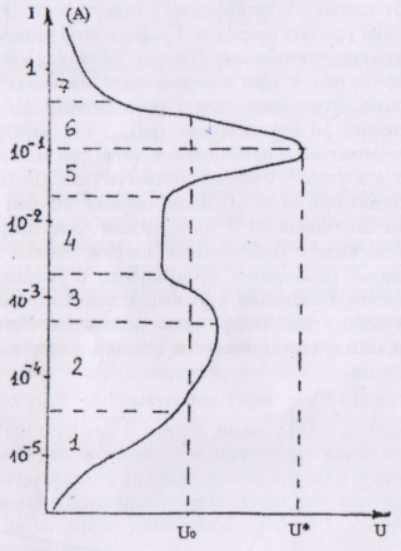
\includegraphics[width=0.4\linewidth]{vax.png}
        \caption{ВАХ газоразрядного диода.}
        \label{img_}
    \end{figure}

\section*{\textbf{Ход работы}}
\addcontentsline{toc}{section}{Ход работы}
\begin{enumerate}
    \item Был включён компьютер и подано питание на установку.
    \item Установка приведена в рабочее состояние. Все краны открыты, внутри везде атмосферное давление. Колбу на установке подсоединена к
источнику напряжения.

    \item Был включён источник напряжения, терморезистивный вакууметр В2,
регулятор газового потока FC и установлен начальный поток газа
равный 100 sccm.

    \item Был включён форвакуумный насос для откачки воздуха до установления постоянного давления.

    \item Была снята зависимость напряжения газоразрядного промежутка от
давления в колбе. Результаты занесены в таблицу 1.




\item По полученным данным был построен график соответствующей зависимости.
Погрешности приборов принимаются равными последнему
разряду.    % P0 - давление, соответствующее минимальному напряжению.
	
\item В камере было установлено давление, соответствующее минимальному
значению напряжения (0,229 торр), и снята ВАХ стабиловольта. И ещё одна ВАХ была снята для давления 0,065 торр.
Результаты занесены в таблицы 2 и 3, построены графики соотетствующих
зависимостей (рисунки 4 -- 6).





\begin{table}[H]
\centering
\begin{tabular}{|c|c|c|c|c|c|c|c|c|c|c|}
\hline
$P,\ 10^{-3} $ торр & 2000 & 1750 & 1000 & 229 & 148 & 125 & 103 & 90 & 78  & 65  \\ \hline
$U,\ 10^{-2}\ $ кВ & 90   & 80   & 70   & 61  & 68  & 74  & 85  & 96 & 108 & 127 \\ \hline
\end{tabular}
\caption{Зависимость напряжения газоразрядного промежутка от давления воздуха.}
\label{table_air1}

\end{table}


\begin{figure}[H]
	\center{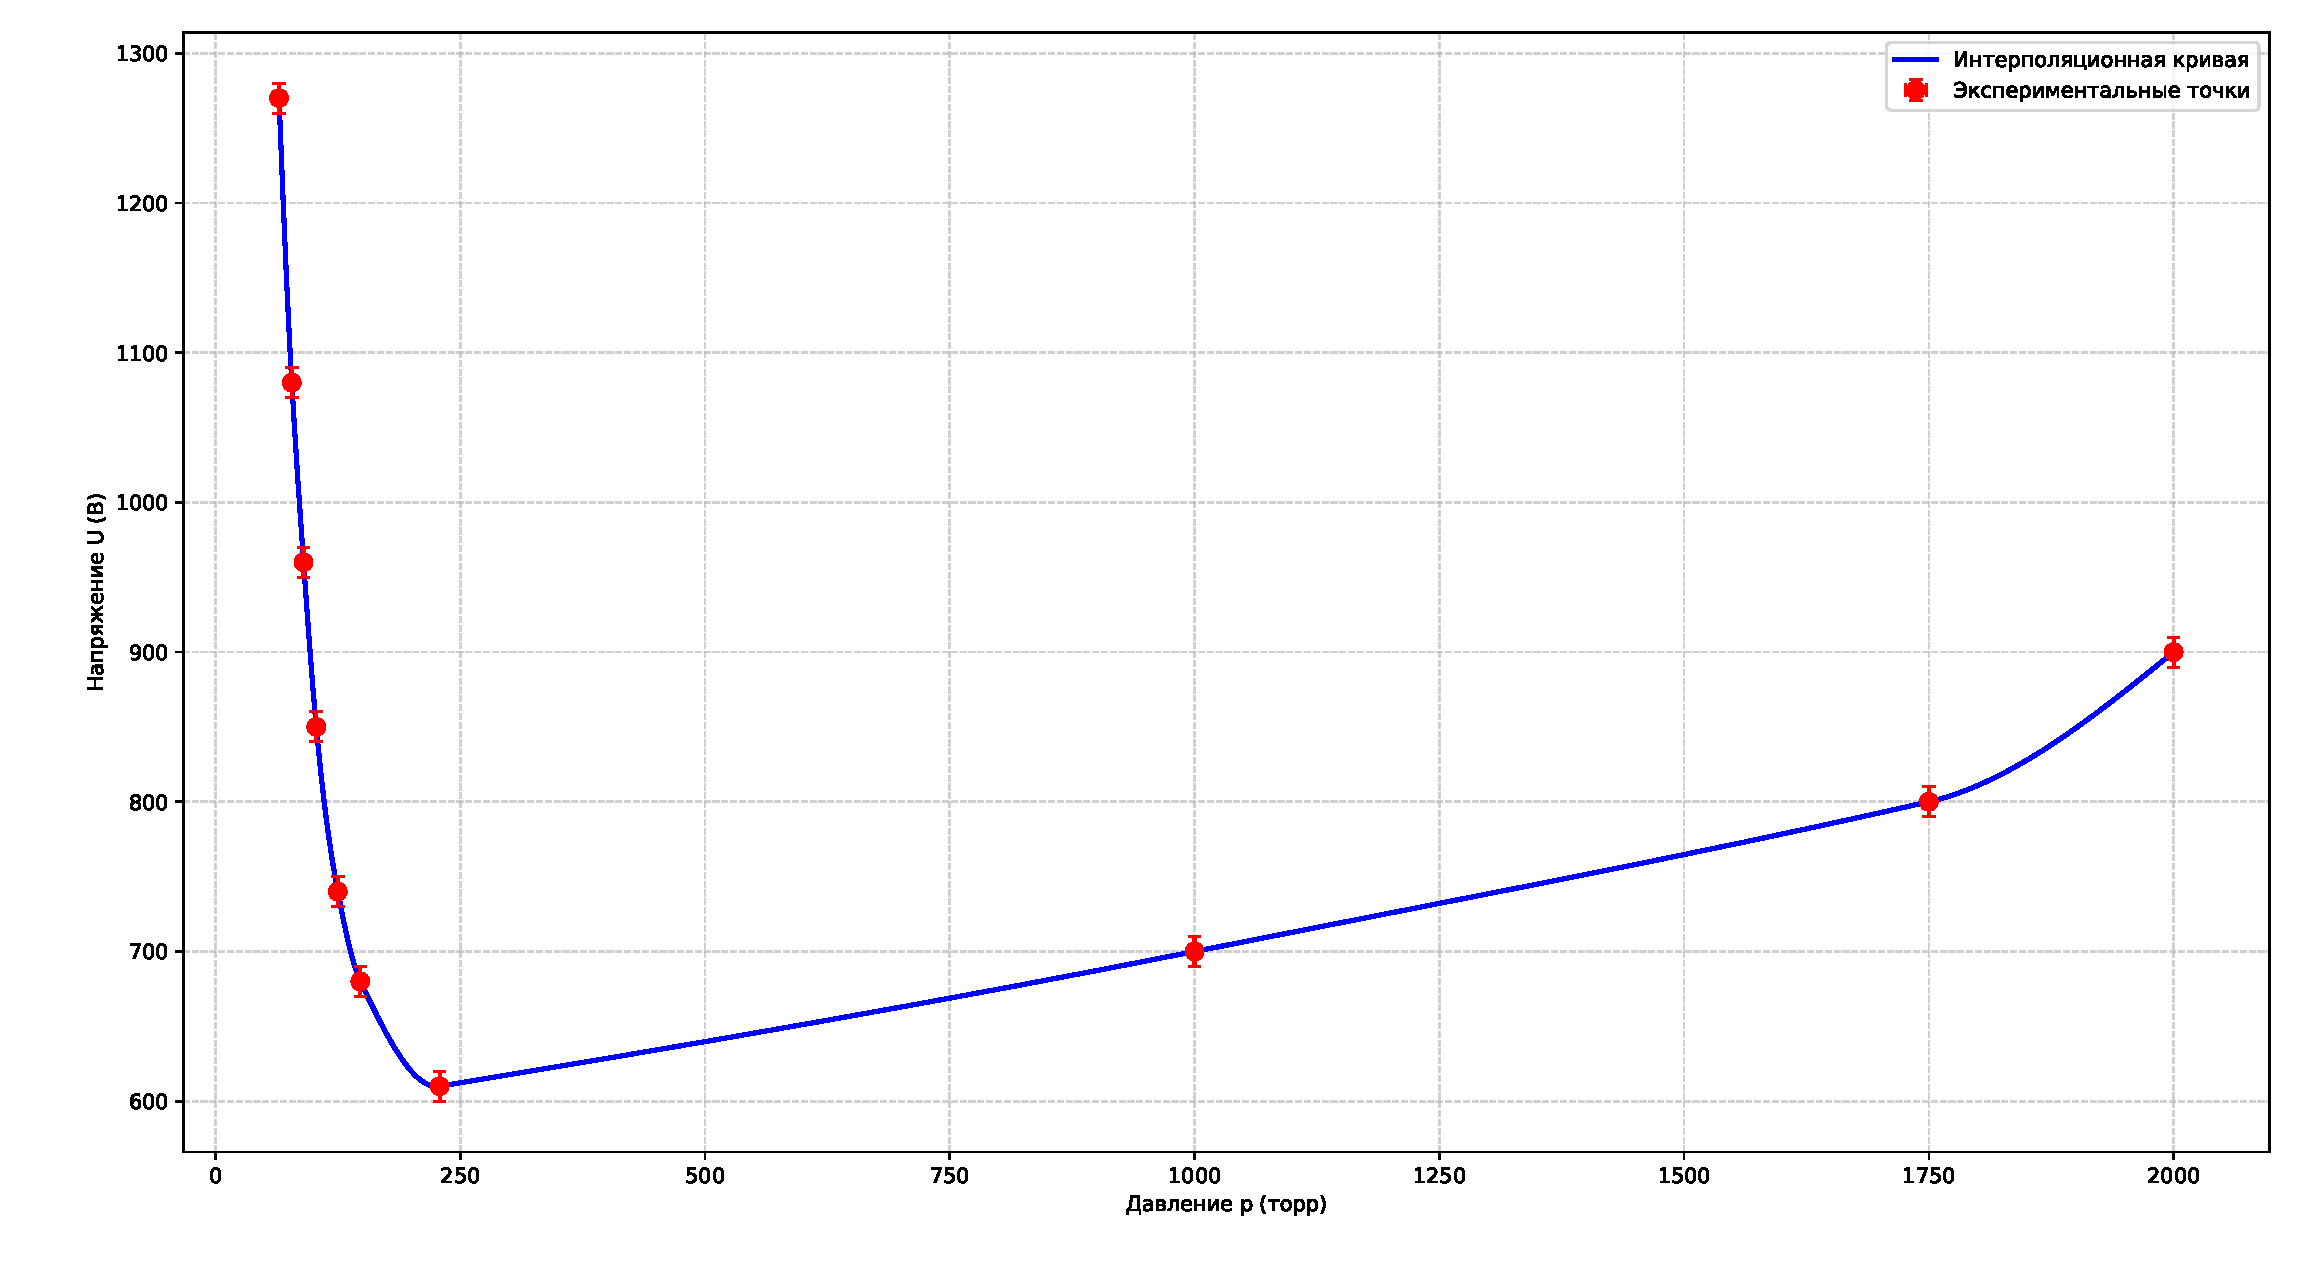
\includegraphics[scale=0.5]{Воздух.pdf}}
    \caption{График зависимости напряжения газоразрядного промежутка от давления
    воздуха в колбе (кривая Пашена).}
    \label{img_1}
\end{figure}


\begin{table}[H]
    \centering
\begin{tabular}{|c|c|c|c|c|c|c|c|c|c|c|}
\hline
$U,\ 10^{-2}\ $ кВ & 59 & 59 & 59 & 60 & 61 & 61 & 62 & 64 & 68 & 67 \\ \hline
$I,\ 10^{-4}$ A    & 19 & 17 & 15 & 13 & 11 & 9  & 7  & 5  & 3  & 1  \\ \hline
\end{tabular}
        \caption{ВАХ стабиловольта для воздуха при давлении 0,229 торр.}
        \label{table_air2}
\end{table}

\begin{table}[H]
    \centering
\begin{tabular}{|c|c|c|c|c|c|c|c|c|c|c|}
\hline
$U,\ 10^{-2}\ $ кВ & 122 & 120 & 117 & 118 & 124 & 125 & 122 & 120 & 118 & 115 \\ \hline
$I,\ 10^{-4}$ A    & 19  & 17  & 15  & 13  & 11  & 9   & 7   & 5   & 3   & 1   \\ \hline
\end{tabular}
        \caption{ВАХ стабиловольта для воздуха при давлении 0,065 торр.}
        \label{table_air3}
\end{table}

\begin{figure}[H]
	\center{
\includegraphics[scale=0.5]{ВАХ 11.pdf}}
    \caption{ВАХ стабиловольта для воздуха при давлении 0,229 торр.}
    \label{img_4}
\end{figure}

\begin{figure}[H]
	\center{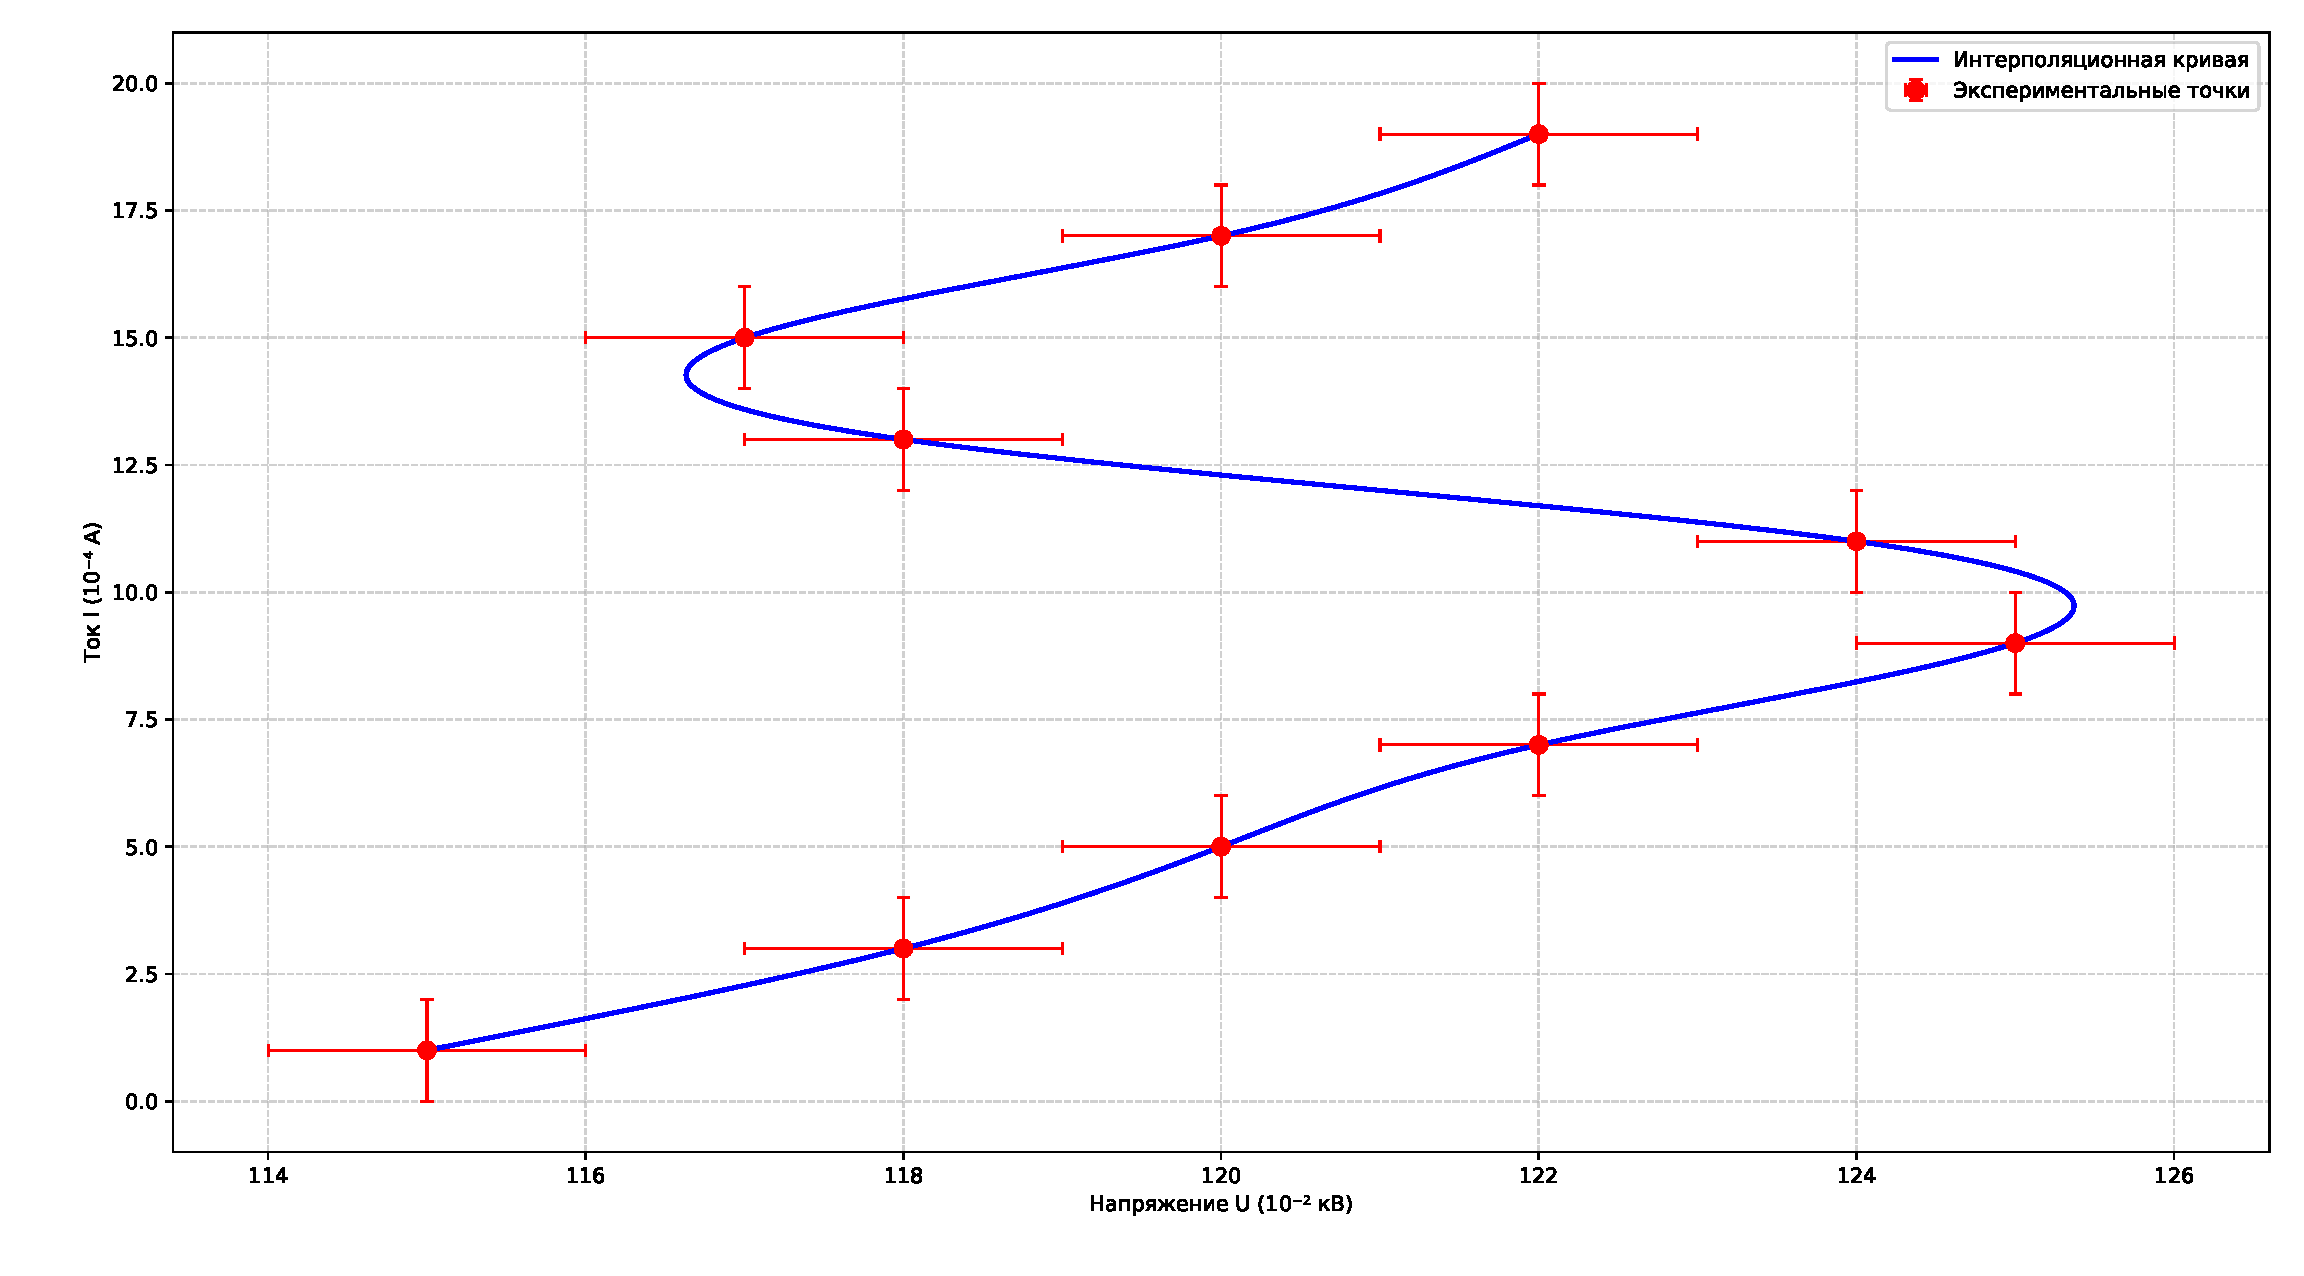
\includegraphics[scale=0.5]{ВАХ 12.pdf}}
    \caption{ВАХ стабиловольта для воздуха при давлении 0,065 торр.}
    \label{img_5}
\end{figure}

\begin{figure}[H]
	\center{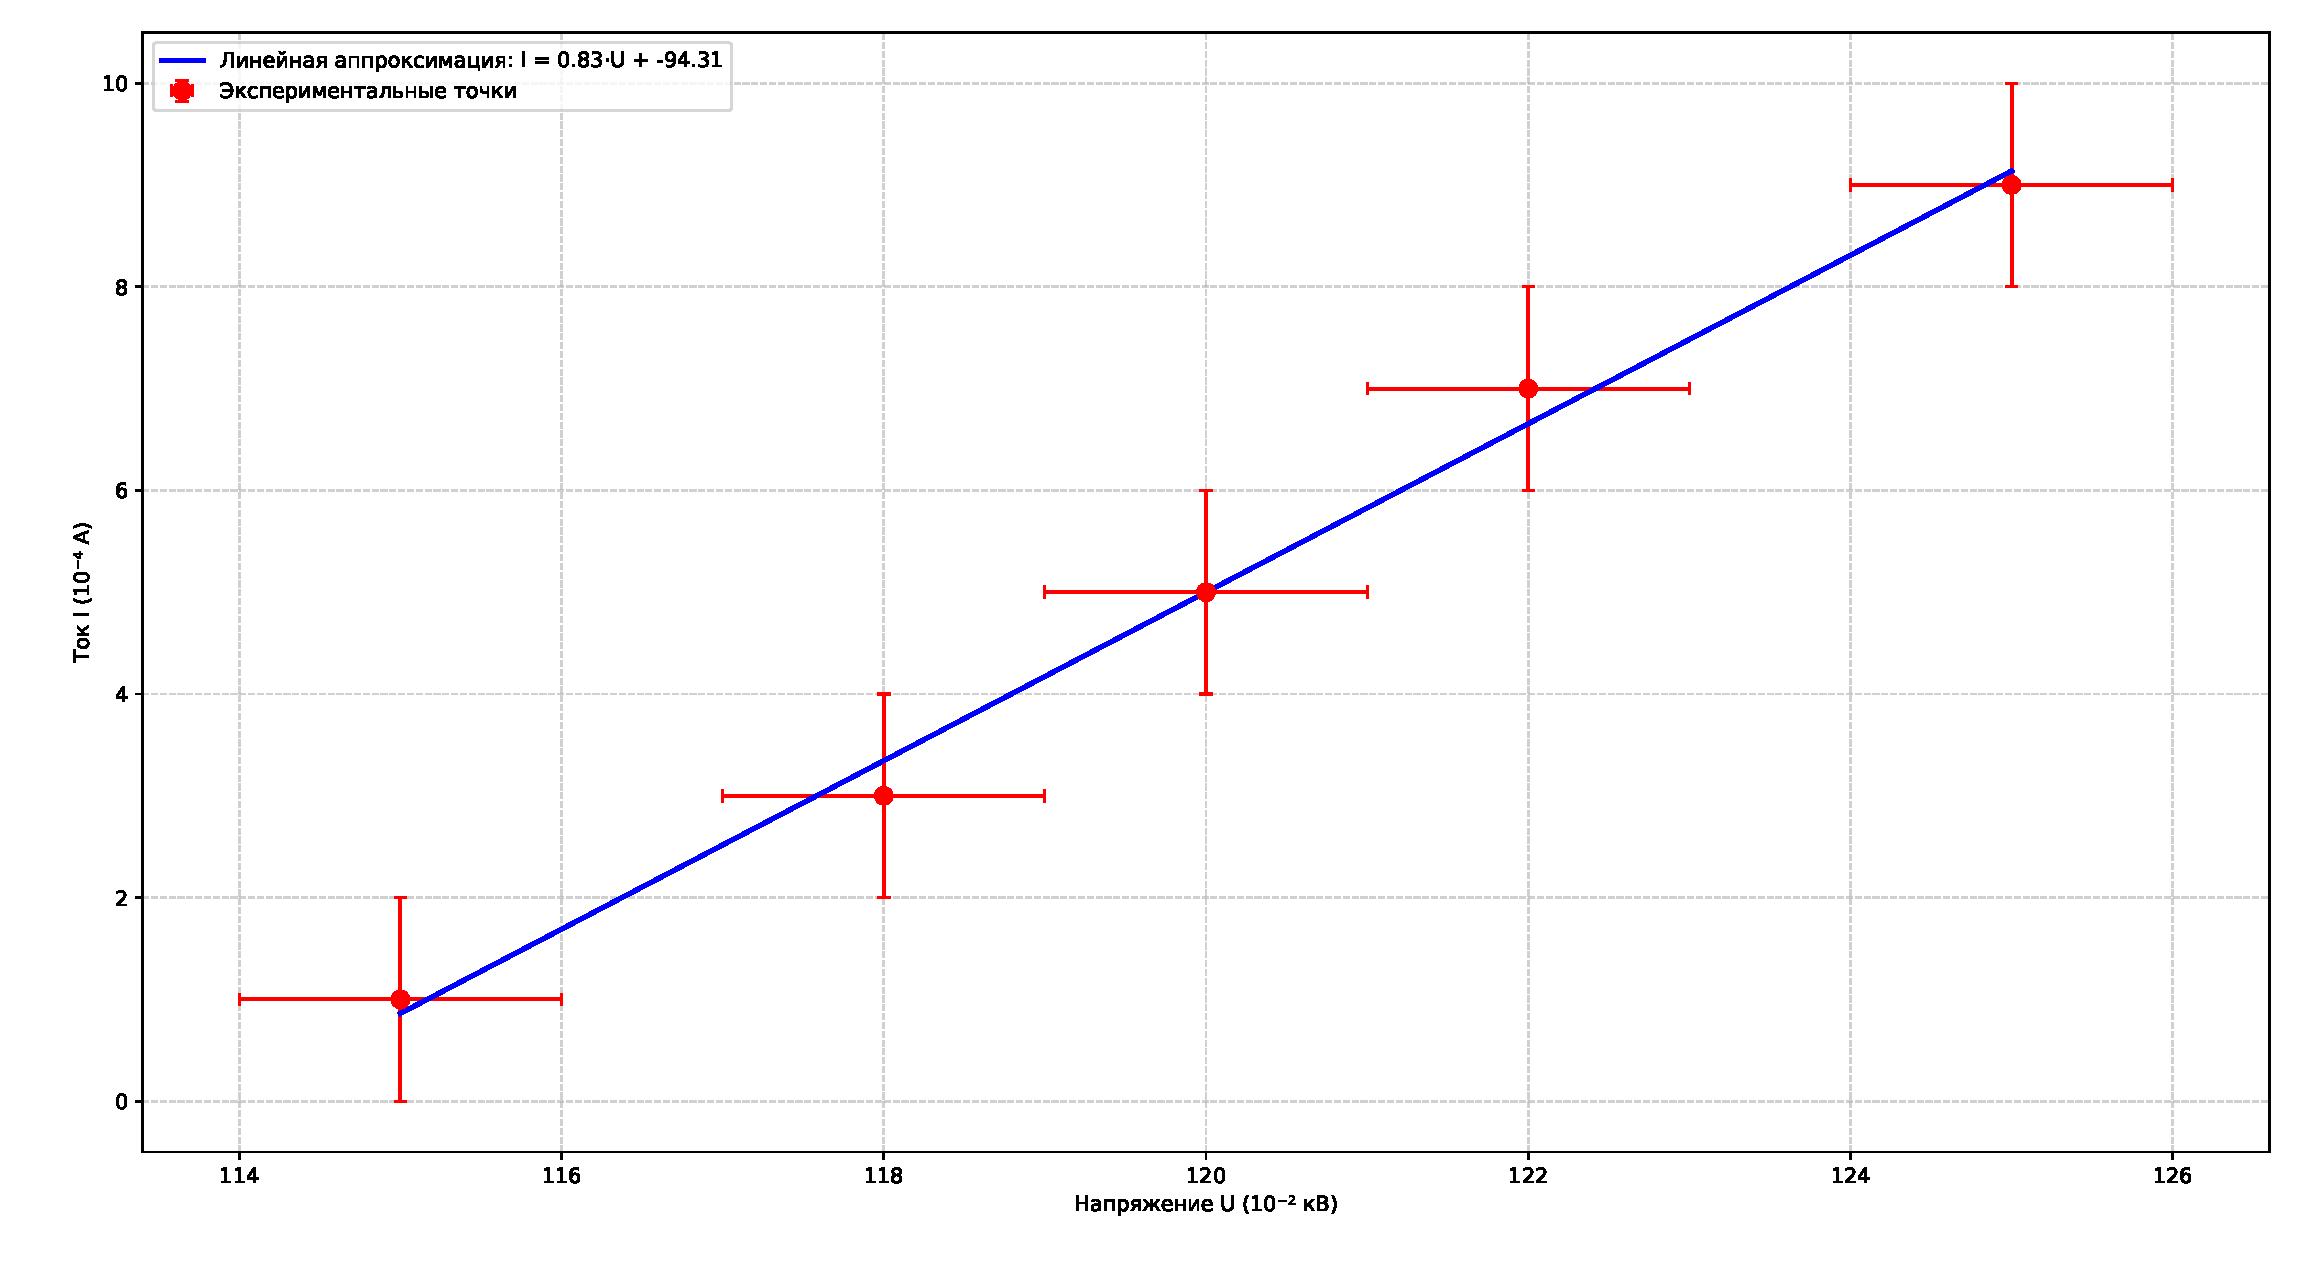
\includegraphics[scale=0.5]{ВАХ 13.pdf}}
    \caption{Линейная часть ВАХ стабиловольта для воздуха при давлении 0,065 торр.}
    \label{img_6}
\end{figure}


\item Воздух в системе был заменён аргоном и повторены действия п. 5) - 7):

\begin{table}[H]
    \centering
\begin{tabular}{|c|c|c|c|c|c|c|c|c|c|c|}
\hline
$P,\ 10^{-3} $ торр & 2420 & 1410 & 220 & 196 & 178 & 128 & 91 & 58 & 68 & 67 \\ \hline
$U,\ 10^{-2}\ $ кВ & 50   & 45   & 40  & 40  & 40  & 41  & 41 & 93 & 3  & 1  \\ \hline
\end{tabular}
\caption{Зависимость напряжения газоразрядного промежутка от давления аргона.}
\end{table}

\begin{figure}[H]
	\center{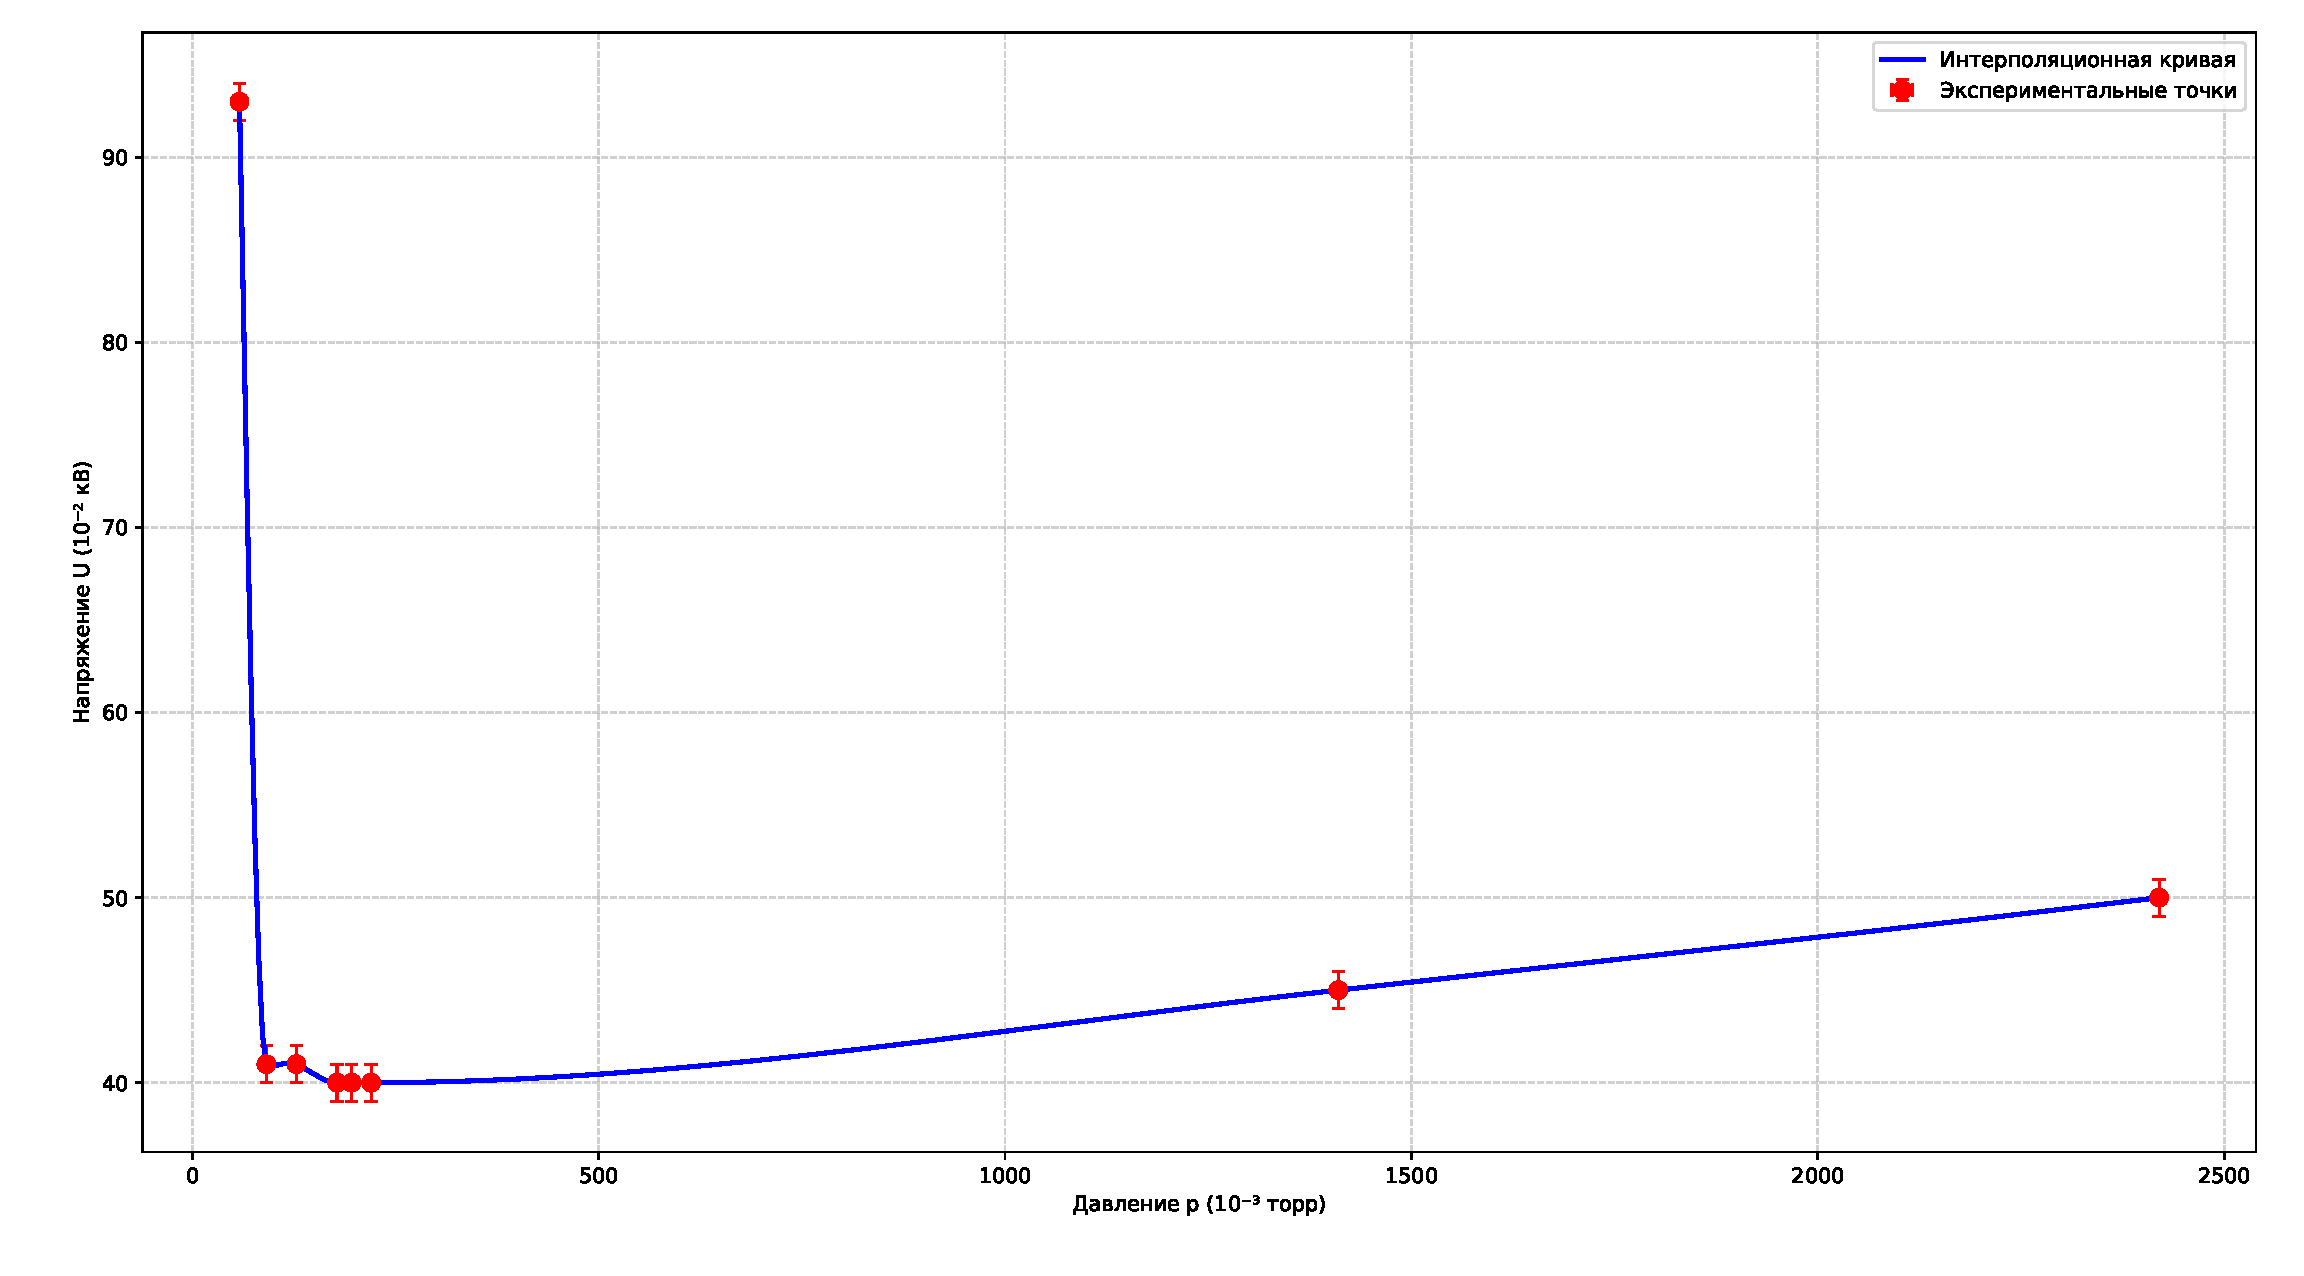
\includegraphics[scale=0.5]{Аргон.pdf}}
    \caption{График зависимости напряжения газоразрядного промежутка от давления
    аргона в колбе (кривая Пашена).}
\end{figure}

\begin{table}[H]
    \centering
\begin{tabular}{|c|c|c|c|c|c|c|c|c|c|c|}
\hline
$U,\ 10^{-2}\ $ кВ & 40 & 40 & 40 & 40 & 42 & 44 & 47 & 48 & 49 & 49 \\ \hline
$I,\ 10^{-4}$ A & 19 & 17 & 15 & 13 & 11 & 9  & 7  & 5  & 3  & 1  \\ \hline
\end{tabular}
\caption{ВАХ стабиловольта для аргона при давлении 0,220 торр.}
\end{table}

\begin{table}[H]
    \centering
\begin{tabular}{|c|c|c|c|c|c|c|c|c|c|c|}
\hline
$U,\ 10^{-2}\ $ кВ & 93 & 93 & 93 & 92 & 89 & 86 & 83 & 80 & 76 & 69 \\ \hline
$I,\ 10^{-4}$ A & 19 & 17 & 15 & 13 & 11 & 9  & 7  & 5  & 3  & 1  \\ \hline
\end{tabular}
\caption{ВАХ стабиловольта для аргона при давлении 0,058 торр.}
\end{table}

\begin{figure}[H]
	\center{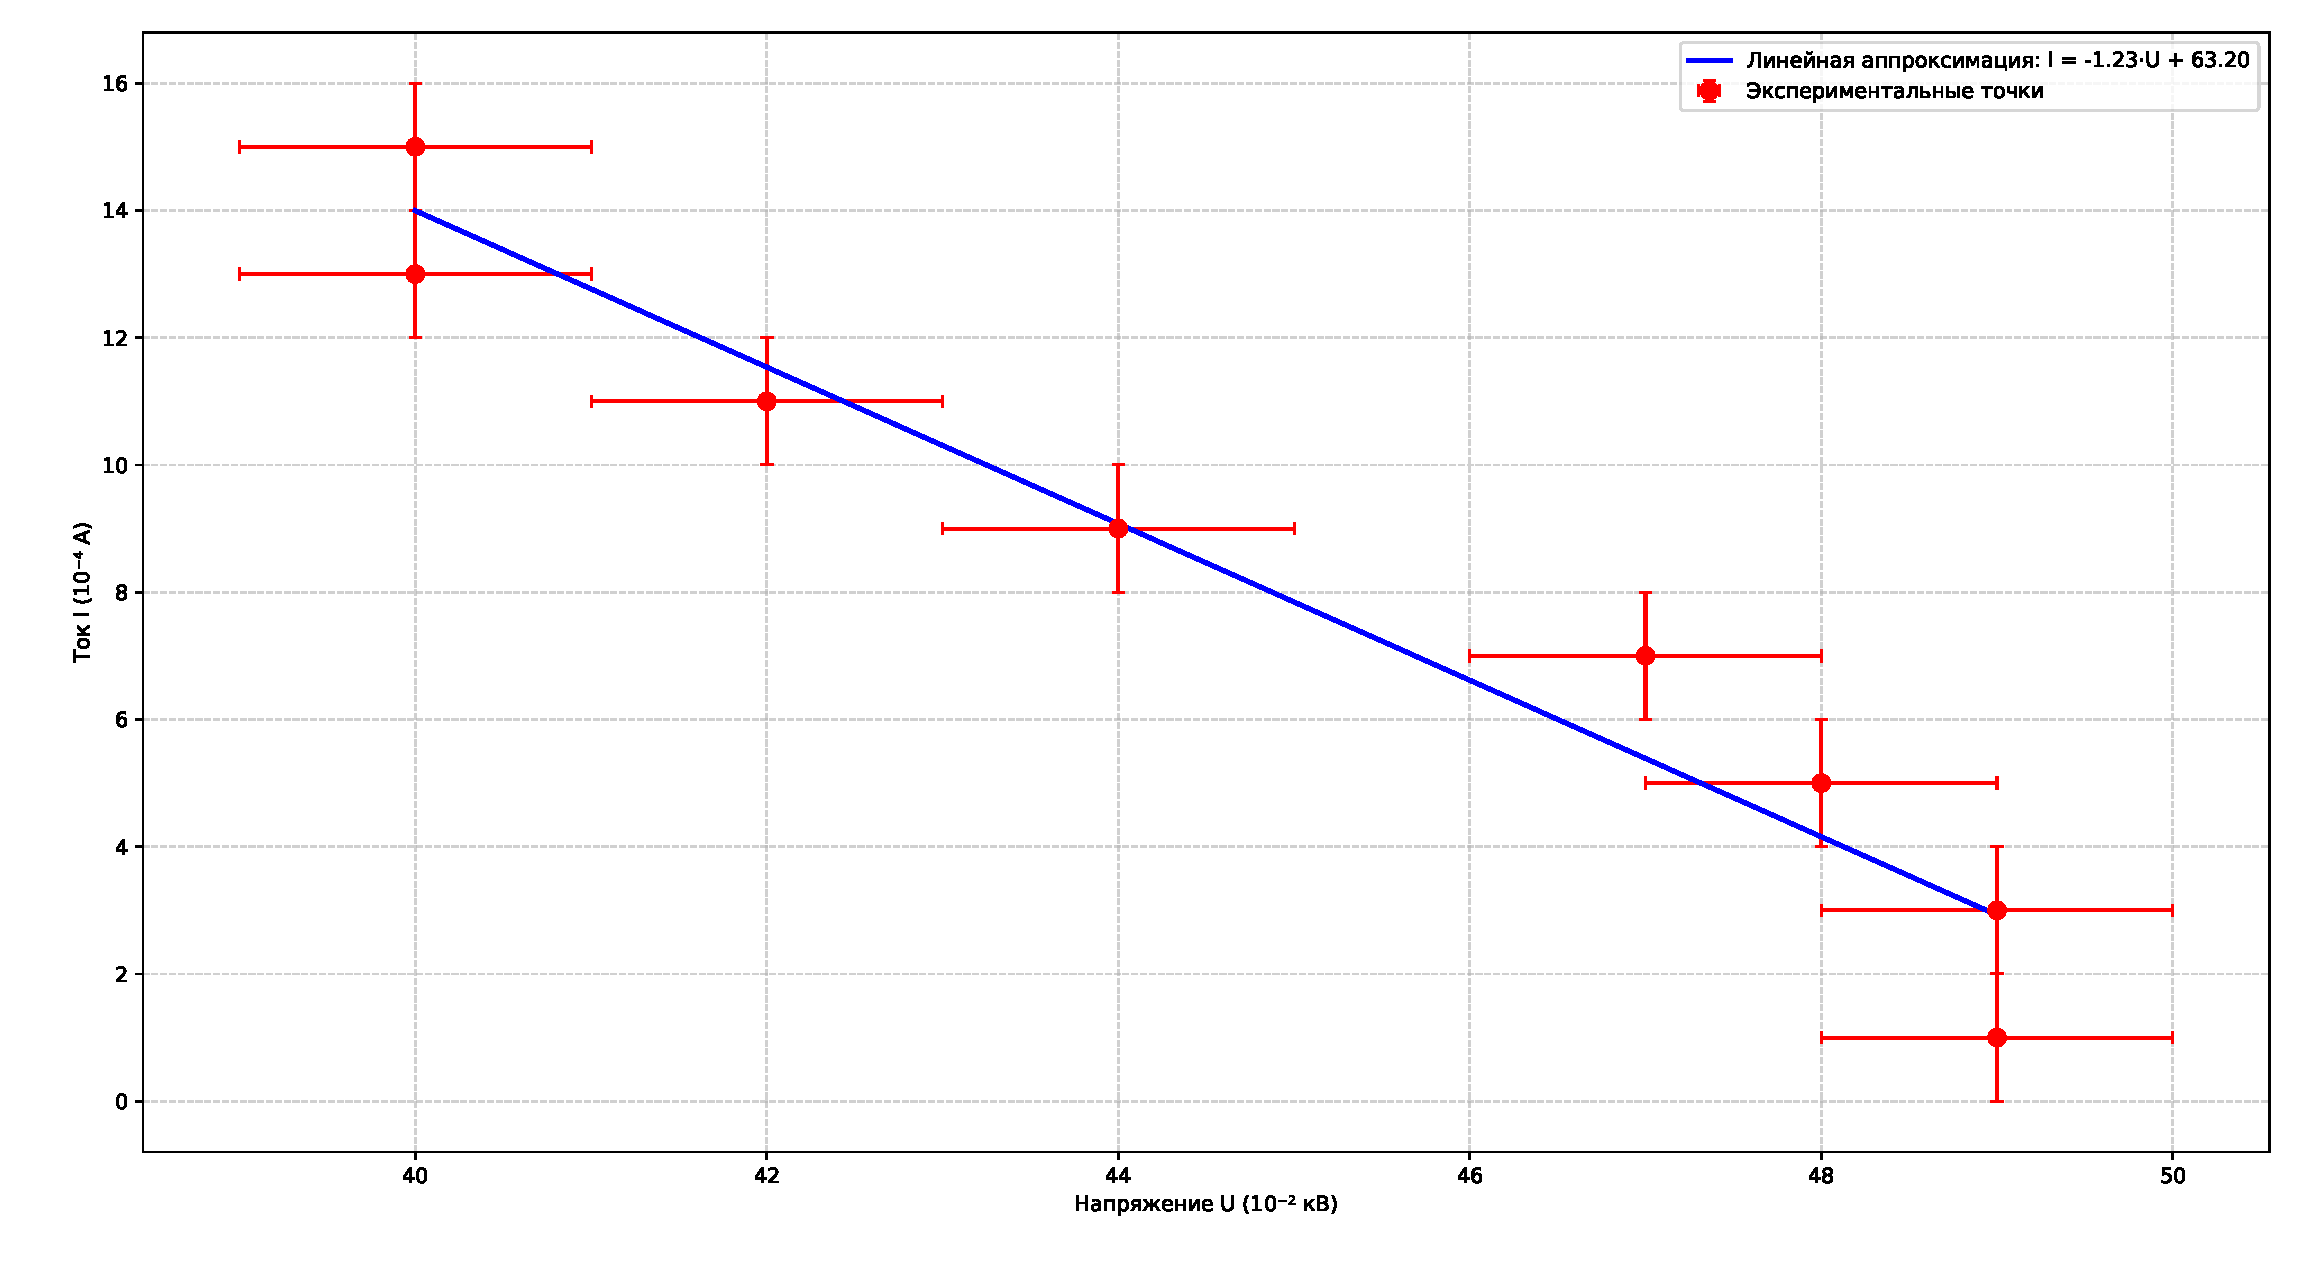
\includegraphics[scale=0.5]{ВАХ 21.pdf}}
    \caption{ВАХ стабиловольта для аргона при давлении 0,220 торр.}
    \label{img_7}
\end{figure}

\begin{figure}[H]
	\center{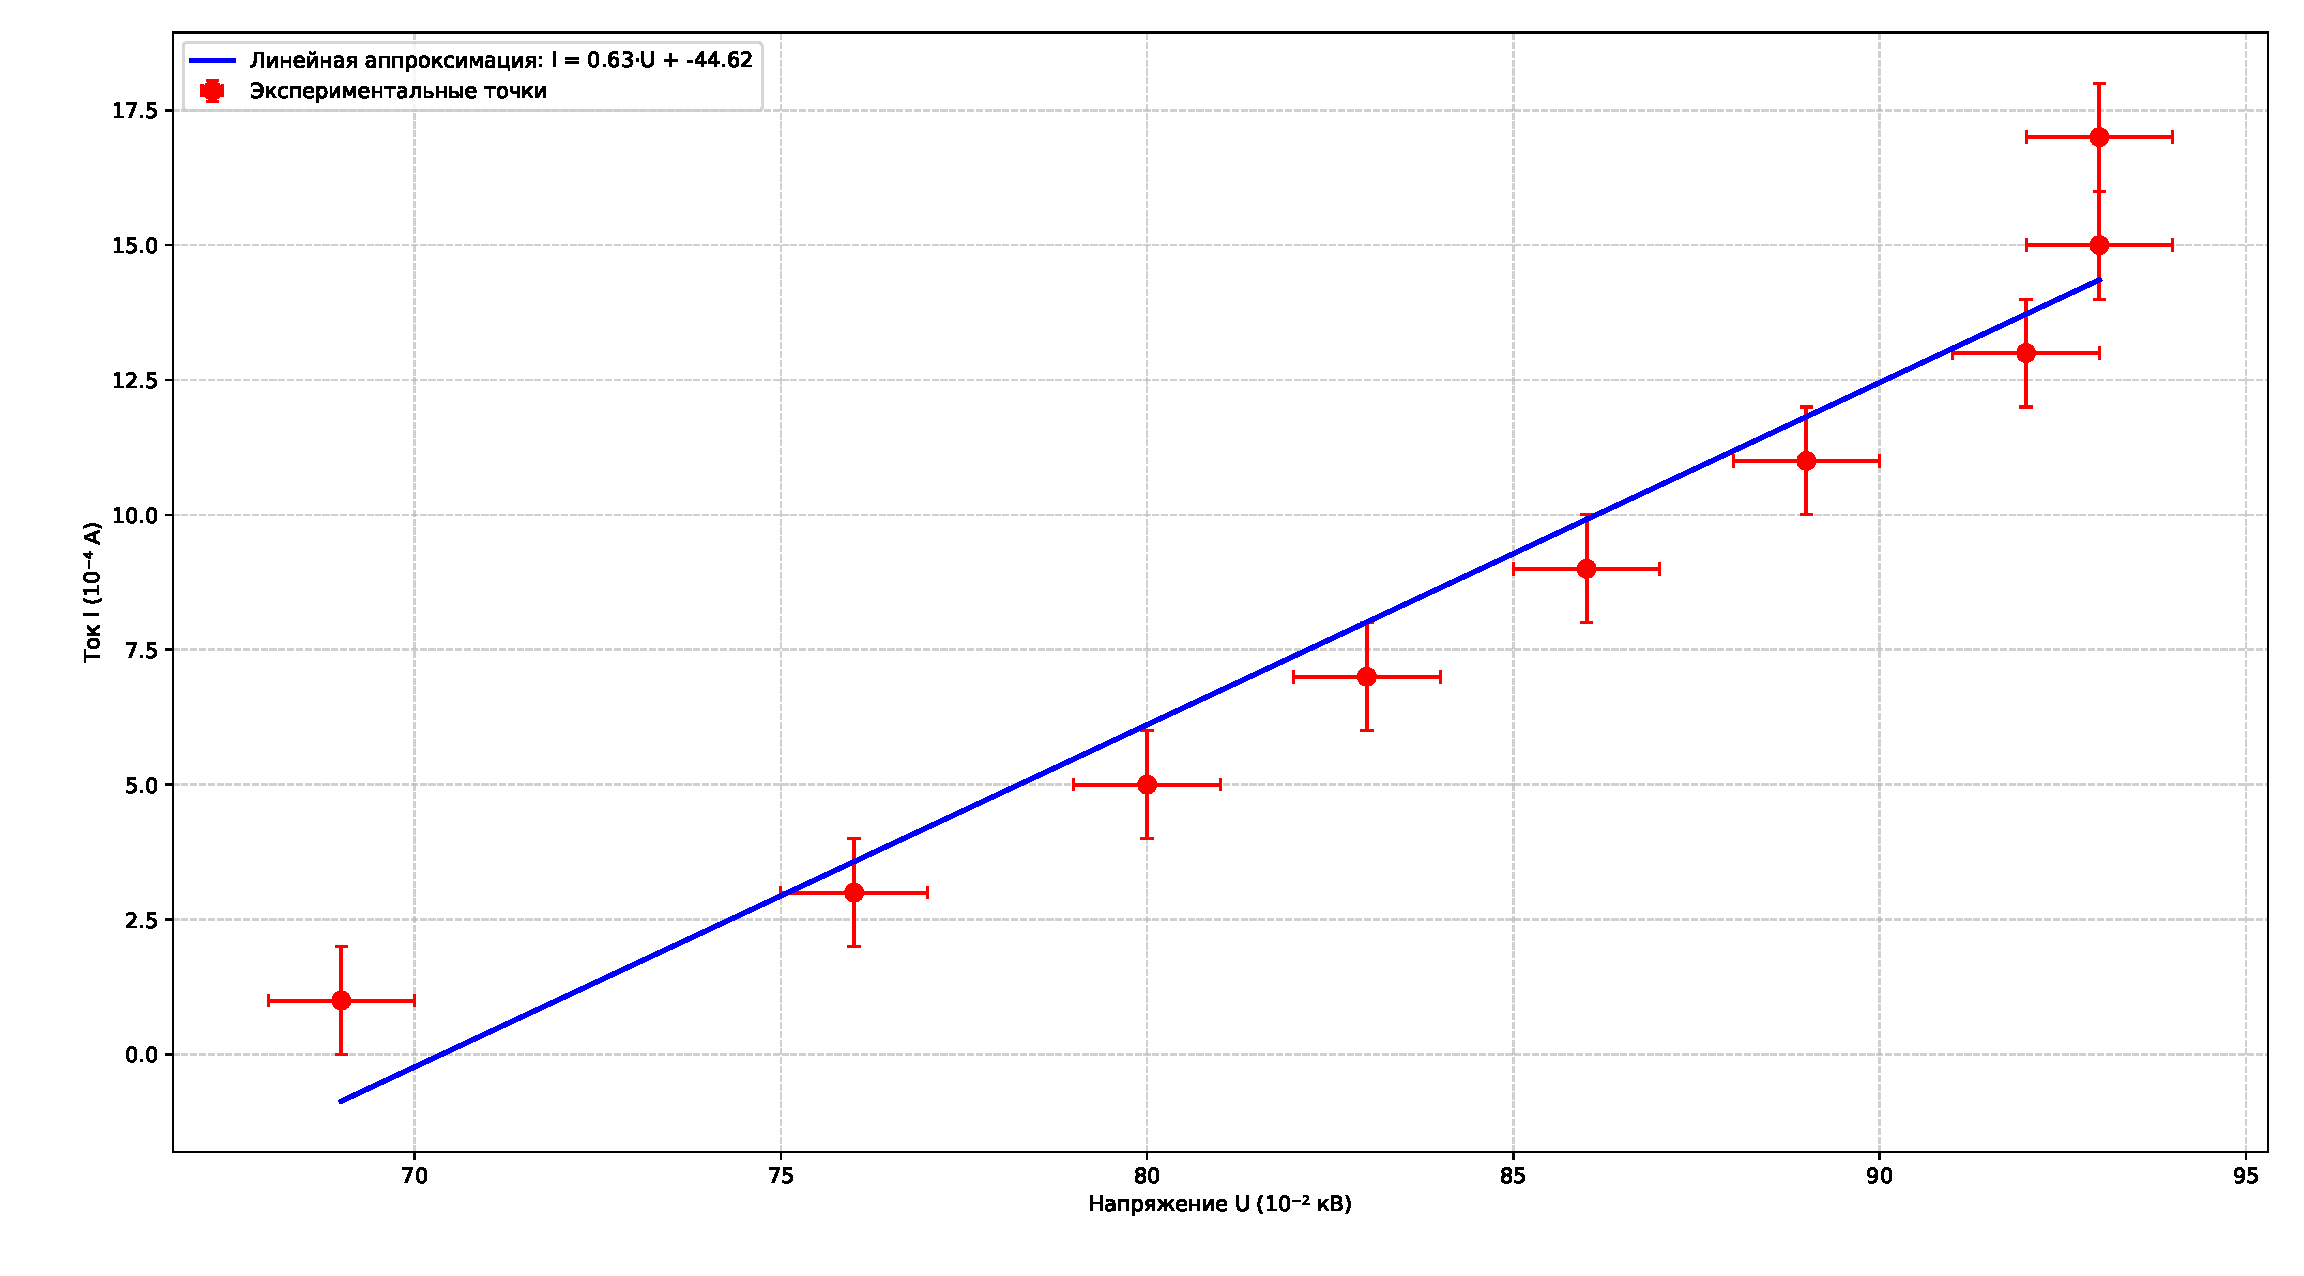
\includegraphics[scale=0.5]{ВАХ 22.pdf}}
    \caption{ВАХ стабиловольта для аргона при давлении 0,058 торр.}
    \label{img_8}
\end{figure}


\item Кривые Пашена и ВАХ воздуха и аргона были помещены на одни графики. Видно, что экспериментальные кривые имеют вид типичных теоретических кривых Пашена, что говорит о применимости теории в нашем случае.

\begin{figure}[H]
	\center{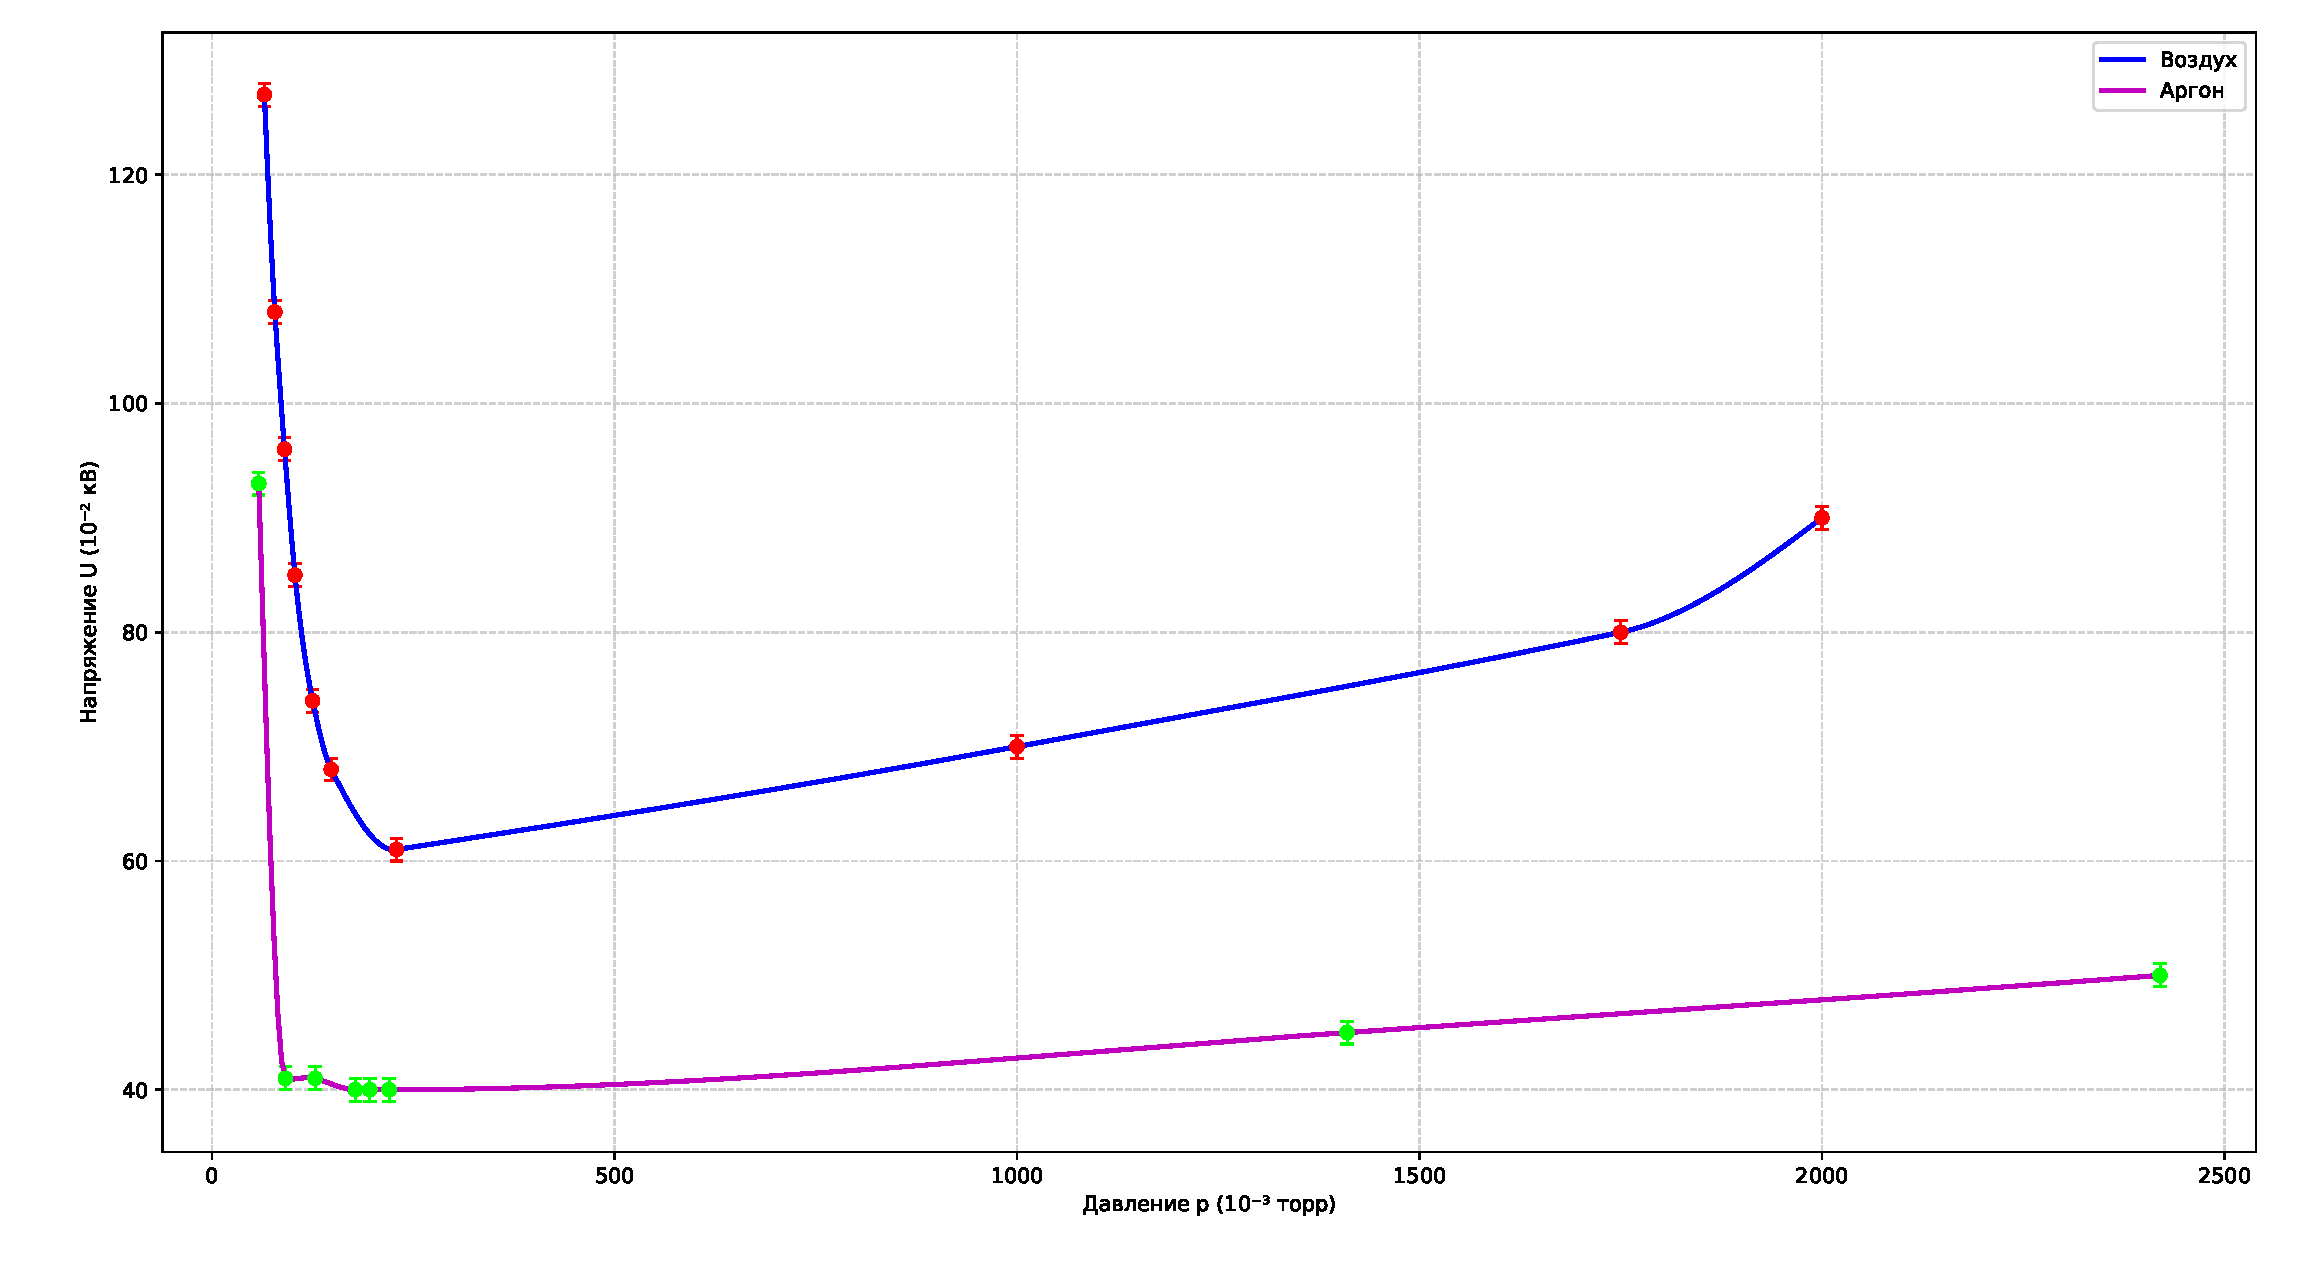
\includegraphics[scale=0.5]{Вместе.pdf}}
    \caption{Кривые Пашена для воздуха и аргона.}
\end{figure}

\begin{figure}[H]
	\center{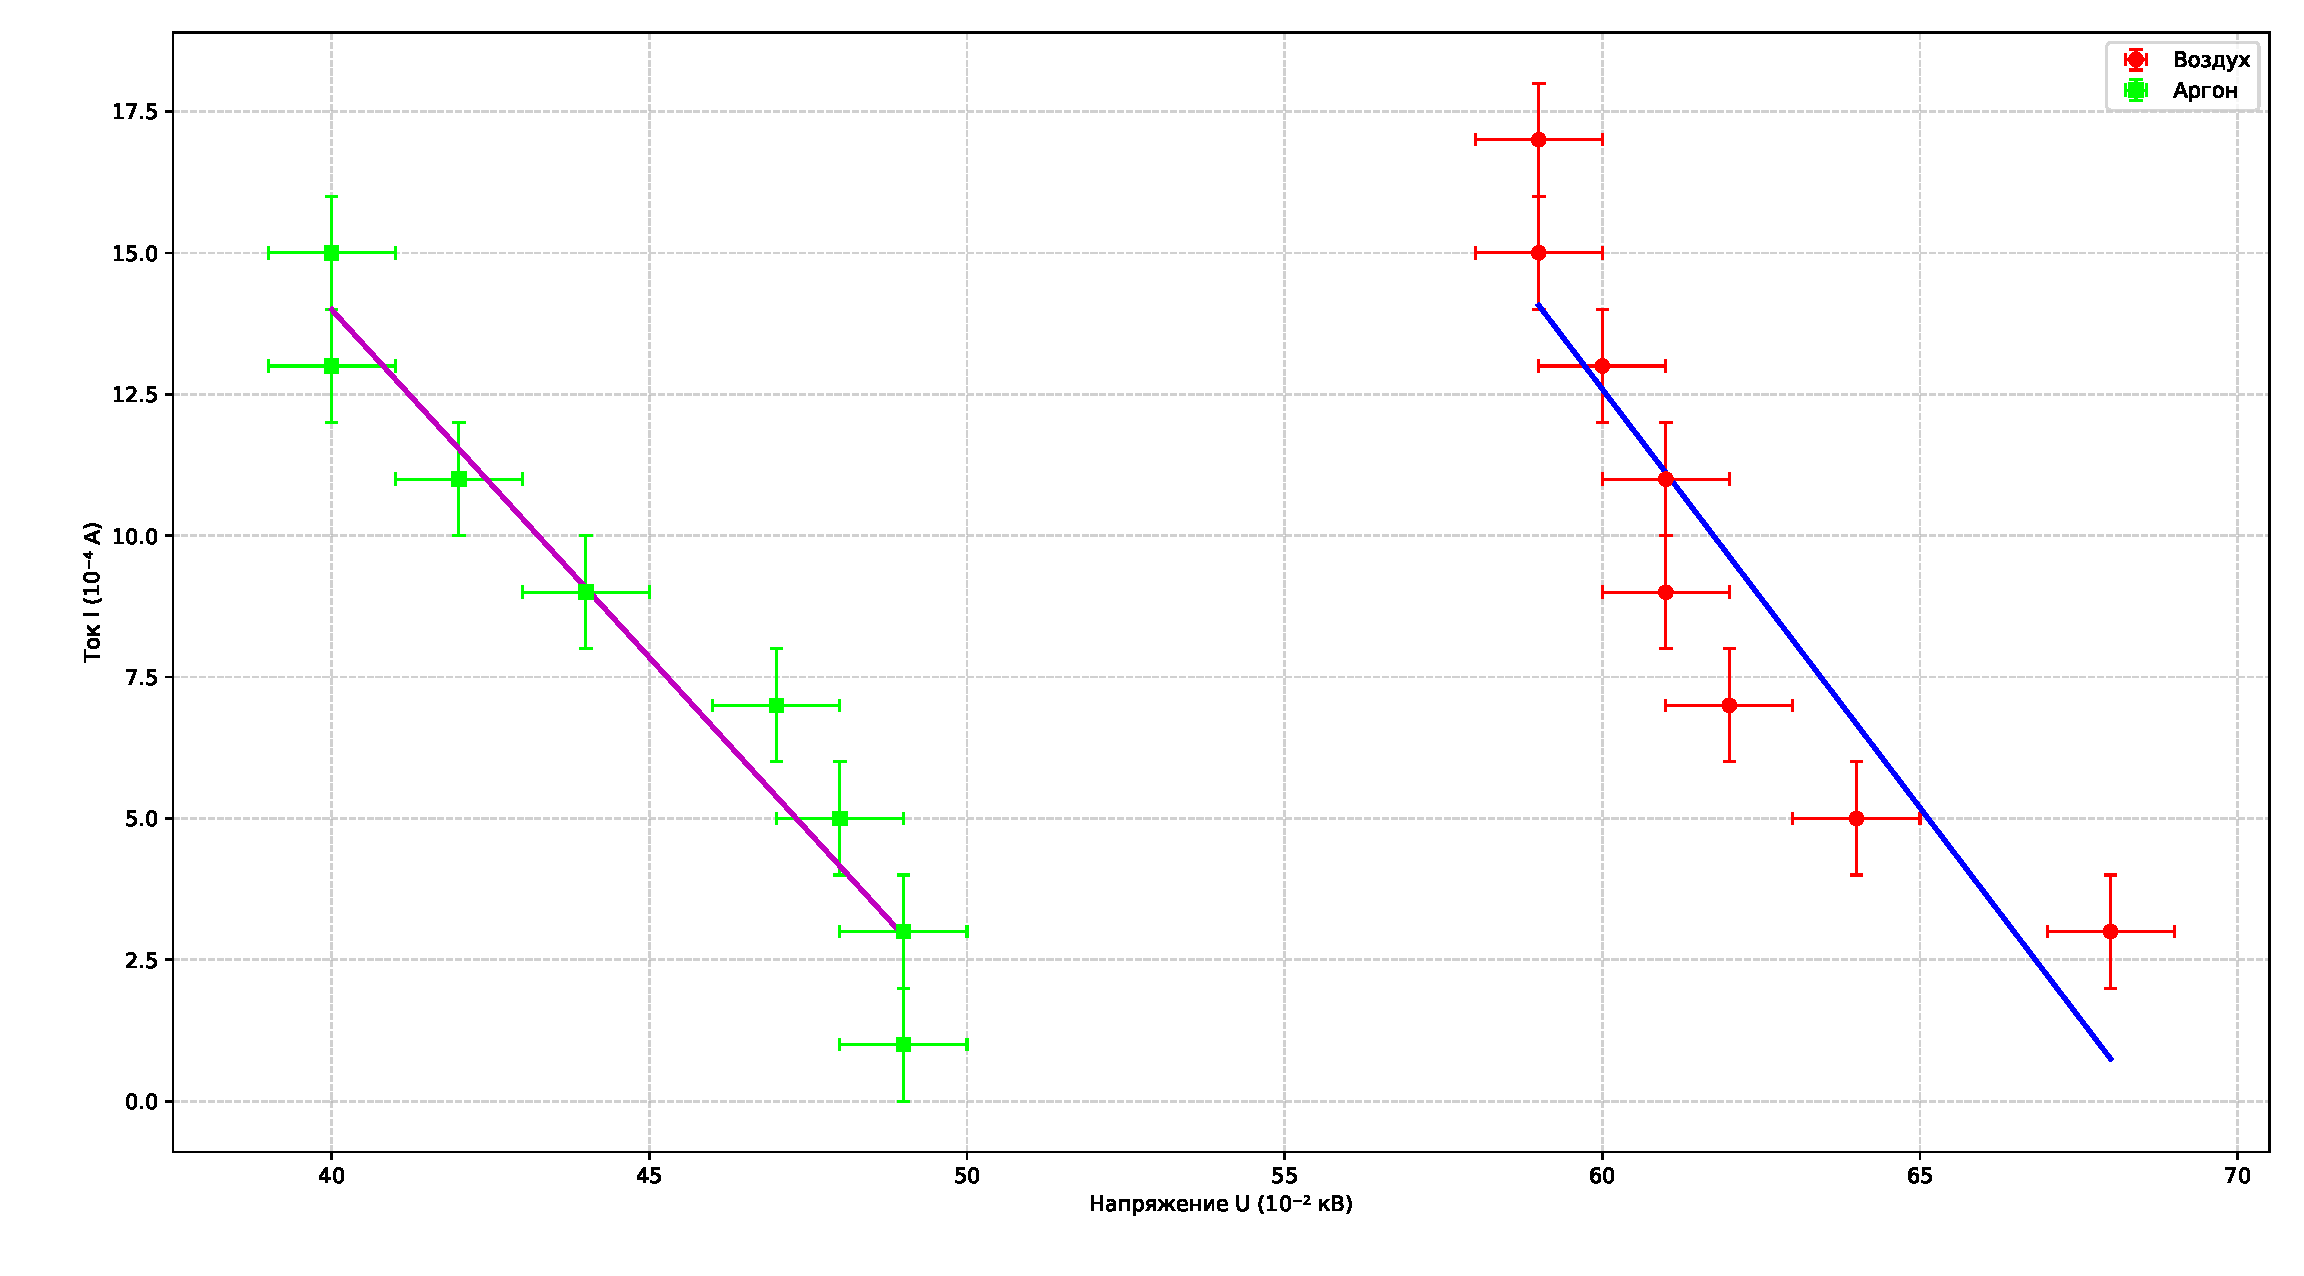
\includegraphics[scale=0.5]{ВАХ вместе.pdf}}
    \caption{Вольт-амперные характеристики стабиловольта для воздуха и аргона.}
\end{figure}

\item По значениям тока и напряжения, а также по общему виду ВАХ
можно утверждать, что они соответствуют участку 3 на рисунке 2, то
есть переходу к тлеющему разряду. Вычисление коэффициента
стабилизации по полученным данным невозможно, поскольку
стабиловольт не вышел на рабочий режим (участок 4 на рисунке 2).


\end{enumerate}

\section*{\textbf{Выводы}}

В результате выполнения работы:

1) Изучены принципы работы газоразрядного стабилизатора напряжения.

2) Получены кривые Пашена при заполнении колбы воздухом и аргоном. Полученные кривые имеют вид, типичный для данной зависимости.

3) Получены вольт-амперные характеристики стабиловольта при заполнении его воздухом и аргоном. По кривым установлено, что режим газового разряда, полученный в работе - переход к тлеющему разряду.


\end{document}